%% start of file `template.tex'.
%% Copyright 2006-2013 Xavier Danaux (xdanaux@gmail.com).
%
% This work may be distributed and/or modified under the
% conditions of the LaTeX Project Public License version 1.3c,
% available at http://www.latex-project.org/lppl/.


\documentclass[10pt,a4paper,sans]{moderncv}        % possible options include font size ('10pt', '11pt' and '12pt'), paper size ('a4paper', 'letterpaper', 'a5paper', 'legalpaper', 'executivepaper' and 'landscape') and font family ('sans' and 'roman')

% moderncv themes
\moderncvstyle{casual}                             % style options are 'casual' (default), 'classic', 'oldstyle' and 'banking'
\moderncvcolor{blue}                               % color options 'blue' (default), 'orange', 'green', 'red', 'purple', 'grey' and 'black'
%\renewcommand{\familydefault}{\sfdefault}         % to set the default font; use '\sfdefault' for the default sans serif font, '\rmdefault' for the default roman one, or any tex font name
%\nopagenumbers{}                                  % uncomment to suppress automatic page numbering for CVs longer than one page

% character encoding
\usepackage[utf8]{inputenc}                       % if you are not using xelatex ou lualatex, replace by the encoding you are using
%\usepackage{CJKutf8}                              % if you need to use CJK to typeset your resume in Chinese, Japanese or Korean
\usepackage{float, graphicx}

% adjust the page margins
\usepackage[scale=0.85]{geometry}
%\setlength{\hintscolumnwidth}{3cm}                % if you want to change the width of the column with the dates
%\setlength{\makecvtitlenamewidth}{10cm}           % for the 'classic' style, if you want to force the width allocated to your name and avoid line breaks. be careful though, the length is normally calculated to avoid any overlap with your personal info; use this at your own typographical risks...

% personal data
\name{Ivan}{Ogasawara}
\title{Open Source Developer}                               % optional, remove / comment the line if not wanted
% \address{street and number}{postcode city}{country}% optional, remove / comment the line if not wanted; the "postcode city" and and "country" arguments can be omitted or provided empty
\phone[mobile]{+591 69757089}                   % optional, remove / comment the line if not wanted
%\phone[fixed]{+2~(345)~678~901}                    % optional, remove / comment the line if not wanted
%\phone[fax]{+3~(456)~789~012}                      % optional, remove / comment the line if not wanted
\email{ivan.ogasawara@gmail.com}                               % optional, remove / comment the line if not wanted
\homepage{https://github.com/xmnlab/}                         % optional, remove / comment the line if not wanted
%\extrainfo{http://lattes.cnpq.br/7764277601641080}                 % optional, remove / comment the line if not wanted
%\photo[64pt][0.4pt]{picture}                       % optional, remove / comment the line if not wanted; '64pt' is the height the picture must be resized to, 0.4pt is the thickness of the frame around it (put it to 0pt for no frame) and 'picture' is the name of the picture file
% \quote{Some quote}                                 % optional, remove / comment the line if not wanted

% to show numerical labels in the bibliography (default is to show no labels); only useful if you make citations in your resume
%\makeatletter
%\renewcommand*{\bibliographyitemlabel}{\@biblabel{\arabic{enumiv}}}
%\makeatother
%\renewcommand*{\bibliographyitemlabel}{[\arabic{enumiv}]}% CONSIDER REPLACING THE ABOVE BY THIS

% bibliography with mutiple entries
%\usepackage{multibib}
%\newcites{book,misc}{{Books},{Others}}
%----------------------------------------------------------------------------------
%            content
%----------------------------------------------------------------------------------
\begin{document}
%\begin{CJK*}{UTF8}{gbsn}                          % to typeset your resume in Chinese using CJK
%-----       resume       ---------------------------------------------------------
\makecvtitle

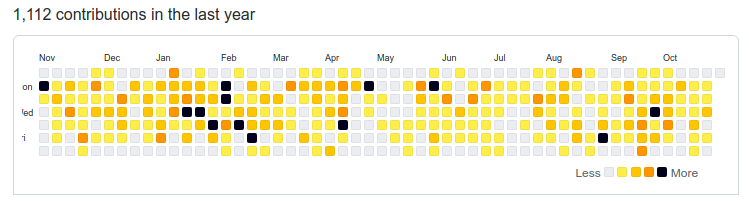
\includegraphics[width=\linewidth]{./images/github.png}

\section{Resumen}
\cventry{}{Analista y desarrollador de programas computacionales con experiencia en proyectos comerciales, gestión pública, ingeniería de transportes, etc. Experiencia en proyectos de investigación científica, análisis de datos, optimización de algoritmos, manipulación de datos georeferenciados y gestión de proyectos}{}{}{}{}{}


\section{Educación}
\cventry{2015--Interrumpida}{Posgrado en ingeniería de transportes y gestión territorial}{Universidade Federal de Santa Catarina}{Florianópolis/Brasil}{\textit{Maestría}}{}  % arguments 3 to 6 can be left empty
\cventry{2004--2005}{Especialización en sistemas de información con énfasis en tecnología de la información}{Faculdade Eniac}{Guarulhos/Brasil}{\textit{Diplomado}}{}

\cventry{2003--2004}{Tecnología en base de datos}{Faculdade Eniac}{Guarulhos/Brasil}{\textit{Pregrado}}{}


\section{Experiencia Laboral}

\cventry{2018--}{Desarrollador en proyectos Open Source}{Quansight}{}{}{Actuación en areas de desarrollo, documentación, devops y/o empaquetamiento de software en proyectos open source como: pytorch, bibliotecas del ecosistema de Jupyter, Ibis, etc. Utilización y desarrollo con tecnologías como: Python, Conda/Conda Constructor, C++, JupyterLab, OmniSciDB, Ibis-Framework, Django, Django-Rest-Framework, GraphQL, Vue.js, Docker, Argo Workflow. Participación en el desarrollo de las fases iniciales del portal \url{openteams.com}.}

\cventry{2016--2018}{Cientista de datos, analista y desarrollador de sistemas}{Independiente/Autónomo}{}{}{Análisis y visualización de datos; Análisis de  literaturas científicas para resolución de problemas; Desarrollo de aplicaciones web para visualización interactiva de datos; Optimización de algoritmos; Manipulación de datos georeferenciados; Despliegue y configuración de servidor MapServer; Utilización de bibliotecas y herramientas Python del stack científico, como: scipy, numpy, numba, pandas, matplotlib, bokeh, rasterio, fiona, jupyter, numexpr, django, flask, conda, etc; Utilización de base de datos PostgreSQL.\newline{}%
\textbf{Participación en los proyectos:}%
\begin{itemize}%
\item Análisis de características visco-elásticas de pavimentos en ensayo en laboratorio;
\item Portal de visualización de incidencia y estimación de influenza en Brasil (\url{github.com/FluVigilanciaBR});
\item Portal de visualización de casos de dengue en Brasil (\url{github.com/AlertaDengue});
\item Creación de paquetes conda de bibliotecas en R (\url{anaconda.org/GlaxoSmithKline});
\end{itemize}}

\cventry{2015--2017}{Open Science and Weigh in Motion Research(OpenWIM)}{Independent Researcher}{}{}{La propuesta del proyecto OpenWIM es crear un entorno digital abierto para apoyar al investigadores del tema de pesaje en movimiento de vehículos pesados (WIM) y mejorar sus prácticas en sus investigaciones por medio de los conceptos de ciencia abierta y por la creación de bibliotecas computaciones basadas en las literaturas de este campo de investigación (\url{github.com/OpenWIM}).}

\cventry{2013--2016}{Analista de Sistemas}{Fundação de Amparo a Pesquisa e Extensão Universitária (FAPEU)}{Florianópolis/Brasil}{}{Participación en proyecto de investigación de pesaje en movimiento de vehículos pesados y desarrollo de algoritmos para análisis de características visco-elásticas de pavimento; Actuación en actividades como: adquisición de datos eléctricos de sensores, procesamiento digital de señales, análisis estadística, aprendizaje automático de máquina, técnicas de optimización de rendimiento, etc.}

\cventry{2011--2013}{Analista Programador de Sistemas}{Cetil Sistemas de Informática S/A, CETIL}{Florianópolis/Brasil}{}{Análisis y desarrollo de sistemas para administración pública.}

\cventry{2011--2011}{Analista de Sistemas}{Victory Consulting (VICTORY)}{São Paulo/Brasil}{}{Desarrollo de herramientas de apoyo a la gestión de seguros de salud y calidad de vida.}

\cventry{2010--2010}{Representante Internacional}{ECELA Spanish Language Schools (ECELA)}{Santiago/Chile}{}{Venta de cursos de inmersión en español en Chile, Argentina y Perú; traducción de materiales publicitarios; desarrollo de páginas WEB.}

\cventry{2007--2009}{Analista de tecnología de información}{Prefeitura Municipal de Guarulhos (PMG)}{Guarulhos/Brasil}{}{Análisis y desarrollo de sistemas para administración pública.}

\cventry{2006--2007}{Profesor}{Centro de Assistência e Promoção Social Nosso Lar (NOSSO LAR)}{Guarulhos/Brasil}{}{Profesor de curso técnico en informática.}

\cventry{2006--2007}{Desarrollador de Sistemas}{Uacari Consultoria de Informática (UACARI)}{Guarulhos/Brasil}{}{Desarrollo de sistemas y sitios WEB y ejecución de actividades comerciales y administrativas.}

\cventry{2005--2005}{Instructor}{Colégio e Faculdade ENIAC (ENIAC)}{Guarulhos/Brasil}{}{Profesor sustituto en disciplinas de tecnología de pregrado. Profesor en clases prácticas en curso técnico en informática.}

\cventry{2005--2005}{Analista de Sistemas}{Vemac Comércio e Serviços LTDA - ME (VEMAC)}{São Paulo/Brasil}{}{Análisis y desarrollo de sistemas para unidades básicas de salud.}

\cventry{2002--2004}{Analista y desarrollador de sistemas}{Colégio Eniac (ENIAC)}{Guarulhos/Brasil}{}{Desarrollo de sistemas y sitios WEB para gestión escolar.}

\cventry{2002--2002}{Analista y desarrollador de Sistemas}{QualityWay (QUALITY WAY)}{São Paulo/Brasil}{}{Desarrollo de sistema interno para gestión de proyectos de auditoría en gestión de recursos y procesos de calidad.}

\section{Eventos realizados}

\cventry{2021--}{Meetups comunidad Open Science Labs}{Organizador}{}{}{Los meetups de la comunidad Open Science Labs tienen como objectivo la difusión de temas como Ciencia Abierta, Código Abierto, Acceso Abierto y herramientas computacionales.}

\cventry{2017--2019}{Meetups comunidad Python La Paz}{Organizador}{}{}{Los meetups realizados en la comunidad Python La Paz tienen como objetivos la difusión de la tecnología Python y la integración entre estudiantes, profesores, desarroladores y empresas que se dedican a este lenguaje.}

\cventry{2015--2016}{4a Conferencia SciPy Latin America}{Presidente}{}{}{La conferencia, realizada entre 16 y 20 de mayo de 2016, tuvo como objetivo fomentar: la ciencia; la adopción de la informática como herramienta de estudio científico y; el uso de Python como principal herramienta informática en la ciencia}

\section{Languages}
\cvitemwithcomment{Portugués}{Nativo}{}
\cvitemwithcomment{Español}{Fluído}{}
\cvitemwithcomment{Inglés}{Avanzado}{}
\cvitemwithcomment{Italiano}{Básico}{}

%Portugués (Nativo) - Español (Fluente) - Inglés (Intermedio) - Italiano  (Intermedio).

%\section{Computer skills}
%\cvdoubleitem{category 1}{XXX, YYY, ZZZ}{category 4}{XXX, YYY, ZZZ}
%\cvdoubleitem{category 2}{XXX, YYY, ZZZ}{category 5}{XXX, YYY, ZZZ}
%\cvdoubleitem{category 3}{XXX, YYY, ZZZ}{category 6}{XXX, YYY, ZZZ}

%\section{Interests}
%\cvitem{hobby 1}{Description}
%\cvitem{hobby 2}{Description}
%\cvitem{hobby 3}{Description}

\section{Certificados}

\cvlistitem{Compilers. edX/Stanford (2021) }
\cvlistitem{Leading With Effective Communication, Inclusive Leadership Training. edX/Catalyst (2021)}
\cvlistitem{Parallel Computing with Dask. DataCamp (2018)}
\cvlistitem{Deep Learning in Python. DataCamp (2018)}
\cvlistitem{Machine Learning with Python. DataCamp (2018)}
\cvlistitem{Machine Learning with the Experts: School Budgets. DataCamp (2018)}
\cvlistitem{Unsupervised Learning in Python. DataCamp (2018)}
\cvlistitem{Importing \& Managing Financial Data in Python. DataCamp (2018)}
\cvlistitem{Supervised Learning with scikit-learn. DataCamp (2018)}
\cvlistitem{Introduction to Applied Biostatistics: Statistics for Medical Research. Osaka University / EDX (2017)}
\cvlistitem{Intro to Hadoop and MapReduce. Udacity (2016)}
\cvlistitem{Intro to Data Science. Udacity (2014)}
\cvlistitem{Machine Learning: Supervised Learning. Udacity (2014)}
\cvlistitem{Intro to Descriptive Statistics. Udacity (2014)}
\cvlistitem{Design of Computer Programs. Udacity (2012)}

%\section{Extra 2}
%\cvlistdoubleitem{Item 1}{Item 4}
%\cvlistdoubleitem{Item 2}{Item 5\cite{book1}}
%\cvlistdoubleitem{Item 3}{Item 6. Like item 3 in the single column list before, this item is particularly long to wrap over several lines.}

%\section{References}
%\begin{cvcolumns}
%  \cvcolumn{Category 1}{\begin{itemize}\item Person 1\item Person 2\item Person 3\end{itemize}}
%  \cvcolumn{Category 2}{Amongst others:\begin{itemize}\item Person 1, and\item Person 2\end{itemize}(more upon request)}
%  \cvcolumn[0.5]{All the rest \& some more}{\textit{That} person, and \textbf{those} also (all available upon request).}
%\end{cvcolumns}

% Publications from a BibTeX file without multibib
%  for numerical labels: \renewcommand{\bibliographyitemlabel}{\@biblabel{\arabic{enumiv}}}% CONSIDER MERGING WITH PREAMBLE PART
%  to redefine the heading string ("Publications"): \renewcommand{\refname}{Articles}
\nocite{*}
\bibliographystyle{plain}
\bibliography{publications}                        % 'publications' is the name of a BibTeX file

\begin{itemize}
\item  Poster: OpenWIM - Open Science and Weigh in Motion Research. International Conference on Weigh-In-Motion 7. DOI: 10.13140/RG.2.2.19198.48961 (\url{https://www.researchgate.net/publication/311735715_OpenWIM_-_Open_Science_and_Weigh_in_Motion_Research})
\end{itemize}


% Publications from a BibTeX file using the multibib package
%\section{Publications}
%\nocitebook{book1,book2}
%\bibliographystylebook{plain}
%\bibliographybook{publications}                   % 'publications' is the name of a BibTeX file
%\nocitemisc{misc1,misc2,misc3}
%\bibliographystylemisc{plain}
%\bibliographymisc{publications}                   % 'publications' is the name of a BibTeX file

\end{document}


%% end of file `template.tex'.
